\section{Experiments}
\label{experiments}
In mobile voice manipulation applications and in found data cases, it is mandatory to use audio recorded far from the ideal studio conditions, with the possibility of finding background noise.
%
The speaker-adaptive HMM-based paradigm has been found quite robust on mel-cepstrum \cite{karhila_jstsp_14, yamagishi2008robustness} and LSP-based vocoders \cite{yanagisawa2013noise}.
%
Nevertheless, in some vocoding and adaptation techniques noise present in the adaptation data can add background noise and produce distortion in the synthetic speech signal.

A GlottHMM-based speaker-adaptive statistical speech synthesis is built in this project, testing the effects of using noisy data in the adaptation.
%
The different noises included in the adaptation data are: babble noise, factory noise and machine gun noise, with different signal-to-noise ratio (SNR).
%
These noises where artificially added into clean data.
%
The results will be compared to the ones obtained with the STRAIGHT-based system in \cite{karhila_jstsp_14}.

\subsection{Initial Experiments}
\label{experiments_initial}
The use of glottal pulses for HMM-synthesis was originally proposed due to the buzzy voice quality caused by simple excitation \cite{raitio2008hmm}.
%
However, a proper modelling of the glottal pulse shape improves the quality in the case of lower fundamental frequency speakers, while speakers with higher $F_{0}$, such as women, do not benefit from the pulse and the impulse excitation may be adequate for them.
%
This particular behavior is the reason of working with a male average voice model, knowing that glottal inverse filtering approach flaws when synthesizing high-pitched voices.

The first step is testing the performance in analysis-resynthesis of GlottHMM when noisy data is used, in order to see if GlottHMM suffer any huge inconvenient caused by the noise.

\begin{figure}[!htb]
\begin{centering}
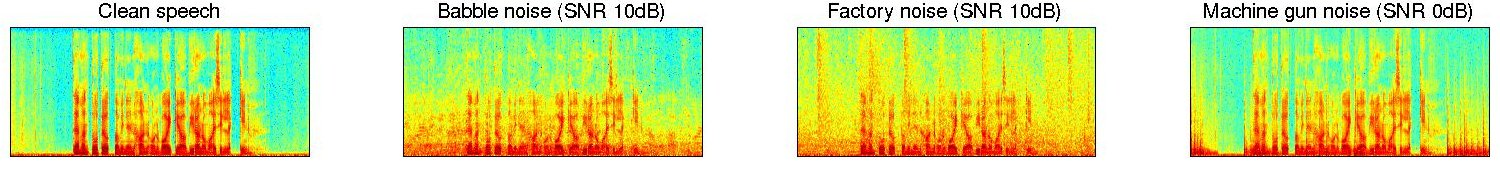
\includegraphics[width=\textwidth]{images/natural_spectra.jpg}
\caption{Natural speech FFT spectra of clean speech, speech with babble noise, factory noise and machine gun noise}
\label{fig:natural_spectra}
\end{centering}
\end{figure}